\documentclass[11pt,a4paper]{article}
\usepackage {amsmath,amsthm}
\usepackage{geometry}
\usepackage{titlesec}
\geometry{a4paper}
\usepackage{natbib}
\usepackage{caption}
\captionsetup{skip=0pt}

%\bibliographystyle{econ}


\usepackage [pdftex]{graphicx}

\usepackage[hidelinks]{hyperref}
%\usepackage[colorlinks=true, urlcolor=blue, pdfborder={0 0 0}]{hyperref}
%\usepackage{comment}
\usepackage{sectsty}
\sectionfont{\fontsize{14}{15}\selectfont}
\subsectionfont{\fontsize{13}{15}\selectfont}

\titleformat*{\section}{\LARGE\bfseries}
\titleformat*{\subsection}{\Large\bfseries}
\usepackage{booktabs}
\usepackage{float}
\usepackage{makecell}
\usepackage{subcaption}
\usepackage{setspace}
\usepackage{placeins}
\usepackage{dcolumn}
\newtheorem{theorem}{Proposition}

\title{\Large Crying Wolf in the Lab\\}
\author{\large Arya Gaduh, Peter McGee, Alexander Ugarov*}
\begin{document}
\maketitle
\onehalfspacing
\begin{abstract}{ }


\vspace{10pt}
\begin{singlespace}

\noindent {\footnotesize{}Keywords: }{\thispagestyle{empty}}
\end{singlespace}
\end{abstract}

\vspace{140pt}
\footnotesize






\onehalfspacing
\normalsize
\newpage
\section{Introduction}

\appendix


\newpage
\section{Tables}
%\begin{table}[h!]\centering
%\def\sym#1{\ifmmode^{#1}\else\(^{#1}\)\fi}
%\caption{xx}
\begin{table}[htbp]\centering
\def\sym#1{\ifmmode^{#1}\else\(^{#1}\)\fi}
\caption{WTP for Information (Discrepancy)}
\begin{tabular}{l*{6}{c}}
\hline\hline
                &\multicolumn{1}{c}{(1)}&\multicolumn{1}{c}{(2)}&\multicolumn{1}{c}{(3)}&\multicolumn{1}{c}{(4)}&\multicolumn{1}{c}{(5)}&\multicolumn{1}{c}{(6)}\\
                &\multicolumn{1}{c}{}&\multicolumn{1}{c}{}&\multicolumn{1}{c}{}&\multicolumn{1}{c}{}&\multicolumn{1}{c}{}&\multicolumn{1}{c}{}\\
\hline
FP costs        &      .17         &     .213\sym{*}  &     .062         &    .0744         &     .338\sym{*}  &      .37\sym{**} \\
                &    (0.1)         &    (0.1)         &    (0.2)         &    (0.2)         &    (0.2)         &    (0.2)         \\
FN costs        &       .3\sym{***}&     .246\sym{***}&     .329\sym{***}&     .314\sym{***}&     .367\sym{***}&      .32\sym{***}\\
                &    (0.1)         &    (0.1)         &    (0.1)         &    (0.1)         &    (0.1)         &    (0.1)         \\
Risk-averse     &                  &                  &  -.00425         &    -.231         &                  &                  \\
                &                  &                  &    (0.3)         &    (0.4)         &                  &                  \\
Risk-averse $\times$ FP costs&                  &                  &     .145         &     .217         &                  &                  \\
                &                  &                  &    (0.2)         &    (0.2)         &                  &                  \\
Risk-averse $\times$ FN costs&                  &                  &   -.0312         &    -.125         &                  &                  \\
                &                  &                  &    (0.1)         &    (0.1)         &                  &                  \\
Accur. beliefs  &                  &                  &                  &                  &     .132         &     .221         \\
                &                  &                  &                  &                  &    (0.3)         &    (0.4)         \\
Accur. beliefs $\times$ FP costs&                  &                  &                  &                  &    -.381\sym{*}  &    -.365         \\
                &                  &                  &                  &                  &    (0.2)         &    (0.2)         \\
Accur. beliefs $\times$ FN costs&                  &                  &                  &                  &    -.133         &    -.145         \\
                &                  &                  &                  &                  &    (0.1)         &    (0.1)         \\
Constant        &    -.111         &     .413\sym{**} &    -.139         &     .463\sym{*}  &    -.173         &     .311         \\
                &    (0.1)         &    (0.2)         &    (0.2)         &    (0.3)         &    (0.2)         &    (0.3)         \\
Prior dummies   &       No         &      Yes         &       No         &      Yes         &       No         &      Yes         \\
\hline
Observations    &      744         &      744         &      690         &      690         &      744         &      744         \\
Adjusted \(R^{2}\)&     0.03         &     0.20         &     0.03         &     0.21         &     0.03         &     0.21         \\
\hline\hline
\multicolumn{7}{l}{\footnotesize Standard errors in parentheses}\\
\multicolumn{7}{l}{\footnotesize \sym{*} \(p<0.10\), \sym{**} \(p<0.05\), \sym{***} \(p<0.01\)}\\
\end{tabular}
\end{table}

%\end{table}

\begin{table}[htbp]\centering
\def\sym#1{\ifmmode^{#1}\else\(^{#1}\)\fi}
\caption{WTP minus Value of Information: demographic determinants}
\begin{tabular}{l*{9}{c}}
\hline\hline
                &\multicolumn{1}{c}{(1)}&\multicolumn{1}{c}{(2)}&\multicolumn{1}{c}{(3)}&\multicolumn{1}{c}{(4)}&\multicolumn{1}{c}{(5)}&\multicolumn{1}{c}{(6)}&\multicolumn{1}{c}{(7)}&\multicolumn{1}{c}{(8)}&\multicolumn{1}{c}{(9)}\\
                &\multicolumn{1}{c}{}&\multicolumn{1}{c}{}&\multicolumn{1}{c}{}&\multicolumn{1}{c}{}&\multicolumn{1}{c}{}&\multicolumn{1}{c}{}&\multicolumn{1}{c}{}&\multicolumn{1}{c}{}&\multicolumn{1}{c}{}\\
\hline
FP costs        &     .558\sym{***}&     .602\sym{***}&     .548\sym{***}&     .475\sym{**} &     .416\sym{**} &      .54\sym{***}&     .485\sym{***}&      .66\sym{***}&     .591\sym{***}\\
                &    (0.1)         &    (0.2)         &    (0.2)         &    (0.2)         &    (0.2)         &    (0.1)         &    (0.1)         &    (0.2)         &    (0.2)         \\
FN costs        &    -.229\sym{*}  &    -.317\sym{*}  &   -.0684         &    -.242         &   -.0701         &    -.295\sym{*}  &   -.0336         &    -.037         &     .223         \\
                &    (0.1)         &    (0.2)         &    (0.2)         &    (0.2)         &    (0.2)         &    (0.2)         &    (0.1)         &    (0.2)         &    (0.2)         \\
Male            &                  &    -.195         &    -.197         &                  &                  &                  &                  &                  &                  \\
                &                  &    (0.4)         &    (0.4)         &                  &                  &                  &                  &                  &                  \\
Male $\times$ FP costs&                  &    -.138         &    -.155         &                  &                  &                  &                  &                  &                  \\
                &                  &    (0.2)         &    (0.2)         &                  &                  &                  &                  &                  &                  \\
Male $\times$ FN costs&                  &     .225         &     .249         &                  &                  &                  &                  &                  &                  \\
                &                  &    (0.3)         &    (0.2)         &                  &                  &                  &                  &                  &                  \\
Stat. class     &                  &                  &                  &    -.161         &    -.179         &                  &                  &                  &                  \\
                &                  &                  &                  &    (0.4)         &    (0.4)         &                  &                  &                  &                  \\
Stat. class $\times$ FP costs&                  &                  &                  &     .138         &     .125         &                  &                  &                  &                  \\
                &                  &                  &                  &    (0.2)         &    (0.2)         &                  &                  &                  &                  \\
Stat. class $\times$ FN costs&                  &                  &                  &    .0192         &     .199         &                  &                  &                  &                  \\
                &                  &                  &                  &    (0.3)         &    (0.2)         &                  &                  &                  &                  \\
$>$23 yrs       &                  &                  &                  &                  &                  &    -.827\sym{**} &    -.785\sym{**} &                  &                  \\
                &                  &                  &                  &                  &                  &    (0.4)         &    (0.3)         &                  &                  \\
$>$23 yrs $\times$ FP costs&                  &                  &                  &                  &                  &     .193         &     .159         &                  &                  \\
                &                  &                  &                  &                  &                  &    (0.3)         &    (0.3)         &                  &                  \\
$>$23 yrs $\times$ FN costs&                  &                  &                  &                  &                  &     .465\sym{**} &     .389         &                  &                  \\
                &                  &                  &                  &                  &                  &    (0.2)         &    (0.3)         &                  &                  \\
Good quiz       &                  &                  &                  &                  &                  &                  &                  &     .347         &     .413         \\
                &                  &                  &                  &                  &                  &                  &                  &    (0.4)         &    (0.4)         \\
Good quiz $\times$ FP costs&                  &                  &                  &                  &                  &                  &                  &    -.194         &    -.178         \\
                &                  &                  &                  &                  &                  &                  &                  &    (0.2)         &    (0.2)         \\
Good quiz $\times$ FN costs&                  &                  &                  &                  &                  &                  &                  &    -.355         &    -.354         \\
                &                  &                  &                  &                  &                  &                  &                  &    (0.3)         &    (0.2)         \\
Constant        &   -.0921         &   -.0115         &     .356         &   .00585         &     .387         &    .0142         &     .363         &    -.279         &    .0568         \\
                &    (0.2)         &    (0.2)         &    (0.3)         &    (0.3)         &    (0.4)         &    (0.2)         &    (0.2)         &    (0.3)         &    (0.3)         \\
Prior dummies   &       No         &       No         &      Yes         &       No         &      Yes         &       No         &      Yes         &       No         &      Yes         \\
\hline
Observations    &      312         &      312         &      312         &      312         &      312         &      312         &      312         &      312         &      312         \\
Adjusted \(R^{2}\)&     0.05         &     0.04         &     0.12         &     0.04         &     0.12         &     0.06         &     0.13         &     0.04         &     0.12         \\
\hline\hline
\multicolumn{10}{l}{\footnotesize Standard errors in parentheses}\\
\multicolumn{10}{l}{\footnotesize \sym{*} \(p<0.10\), \sym{**} \(p<0.05\), \sym{***} \(p<0.01\)}\\
\end{tabular}
\end{table}
 \label{xx}

\begin{table}[htbp]\centering
\def\sym#1{\ifmmode^{#1}\else\(^{#1}\)\fi}
\caption{WTP for Information (different risk aversion)}
\begin{tabular}{l*{6}{c}}
\hline\hline
                &\multicolumn{1}{c}{(1)}&\multicolumn{1}{c}{(2)}&\multicolumn{1}{c}{(3)}&\multicolumn{1}{c}{(4)}&\multicolumn{1}{c}{(5)}&\multicolumn{1}{c}{(6)}\\
                &\multicolumn{1}{c}{$\theta=0$}&\multicolumn{1}{c}{$\theta=0.5$}&\multicolumn{1}{c}{$\theta=1.0$}&\multicolumn{1}{c}{$\theta=1.5$}&\multicolumn{1}{c}{$\theta=2.5$}&\multicolumn{1}{c}{Heterogeneous $\theta$}\\
\hline
FP costs        &     .183         &     .212         &      .21         &     .165         &    .0499         &     .162         \\
                &    (0.1)         &    (0.1)         &    (0.1)         &    (0.1)         &    (0.1)         &    (0.1)         \\
FN costs        &     .212\sym{***}&     .317\sym{***}&     .431\sym{***}&      .53\sym{***}&      .66\sym{***}&     .234\sym{***}\\
                &    (0.1)         &    (0.1)         &    (0.1)         &    (0.1)         &    (0.1)         &    (0.1)         \\
Constant        &     .402\sym{**} &   .00285         &    -.516\sym{***}&    -1.17\sym{***}&    -1.67\sym{***}&   -.0609         \\
                &    (0.2)         &    (0.2)         &    (0.2)         &    (0.2)         &    (0.2)         &    (0.2)         \\
Prior dummies   &      Yes         &      Yes         &      Yes         &      Yes         &      Yes         &      Yes         \\
\hline
Observations    &      594         &      594         &      594         &      594         &      594         &      594         \\
Adjusted \(R^{2}\)&     0.19         &     0.24         &     0.25         &     0.30         &     0.35         &     0.12         \\
\hline\hline
\multicolumn{7}{l}{\footnotesize Standard errors in parentheses}\\
\multicolumn{7}{l}{\footnotesize \sym{*} \(p<0.10\), \sym{**} \(p<0.05\), \sym{***} \(p<0.01\)}\\
\end{tabular}
\end{table}

\begin{table}[htbp]\centering
\def\sym#1{\ifmmode^{#1}\else\(^{#1}\)\fi}
\caption{WTP for Information (different risk aversion)}
\begin{tabular}{l*{5}{c}}
\hline\hline
                &\multicolumn{1}{c}{(1)}&\multicolumn{1}{c}{(2)}&\multicolumn{1}{c}{(3)}&\multicolumn{1}{c}{(4)}&\multicolumn{1}{c}{(5)}\\
                &\multicolumn{1}{c}{$\theta=0$}&\multicolumn{1}{c}{$\theta=0.5$}&\multicolumn{1}{c}{$\theta=1.0$}&\multicolumn{1}{c}{$\theta=1.5$}&\multicolumn{1}{c}{$\theta=2.5$}\\
\hline
FP costs        &     .213\sym{**} &     .246\sym{***}&     .246\sym{***}&     .201\sym{**} &    .0858         \\
                &    (2.3)         &    (2.6)         &    (2.6)         &    (2.1)         &    (0.8)         \\
FN costs        &     .246\sym{***}&     .348\sym{***}&      .46\sym{***}&     .556\sym{***}&     .687\sym{***}\\
                &    (4.2)         &    (5.9)         &    (7.5)         &    (8.8)         &   (10.2)         \\
Constant        &     .413\sym{***}&    .0134         &    -.505\sym{***}&    -1.16\sym{***}&    -1.66\sym{***}\\
                &    (3.4)         &    (0.1)         &   (-4.1)         &   (-9.5)         &  (-12.8)         \\
Prior dummies   &      Yes         &      Yes         &      Yes         &      Yes         &      Yes         \\
\hline
Observations    &      744         &      744         &      744         &      744         &      744         \\
Adjusted \(R^{2}\)&     0.20         &     0.25         &     0.26         &     0.30         &     0.35         \\
\hline\hline
\multicolumn{6}{l}{\footnotesize \textit{t} statistics in parentheses}\\
\multicolumn{6}{l}{\footnotesize \sym{*} \(p<0.10\), \sym{**} \(p<0.05\), \sym{***} \(p<0.01\)}\\
\end{tabular}
\end{table}


\begin{table}[htbp]\centering
\def\sym#1{\ifmmode^{#1}\else\(^{#1}\)\fi}
\caption{Belief Elicitation: Discrepancy}
\begin{tabular}{l*{6}{c}}
\hline\hline
                &\multicolumn{1}{c}{(1)}&\multicolumn{1}{c}{(2)}&\multicolumn{1}{c}{(3)}&\multicolumn{1}{c}{(4)}&\multicolumn{1}{c}{(5)}&\multicolumn{1}{c}{(6)}\\
                &\multicolumn{1}{c}{}&\multicolumn{1}{c}{}&\multicolumn{1}{c}{}&\multicolumn{1}{c}{}&\multicolumn{1}{c}{}&\multicolumn{1}{c}{}\\
\hline
FN rate         &     .016         &     .016         &    -.014         &    -.014         &   -.0562         &   -.0554         \\
                &    (0.1)         &    (0.1)         &    (0.1)         &    (0.1)         &    (0.1)         &    (0.1)         \\
FP rate         &     .919\sym{***}&     .919\sym{***}&     1.07\sym{***}&     1.07\sym{***}&     1.05\sym{***}&     1.05\sym{***}\\
                &    (0.1)         &    (0.1)         &    (0.1)         &    (0.1)         &    (0.1)         &    (0.1)         \\
Good quiz       &                  &                  &    .0469         &    .0673         &                  &                  \\
                &                  &                  &    (0.0)         &    (0.0)         &                  &                  \\
Good quiz $\times$ FN rate&                  &                  &    .0463         &    .0464         &                  &                  \\
                &                  &                  &    (0.1)         &    (0.1)         &                  &                  \\
Good quiz $\times$ FP rate&                  &                  &    -.286\sym{*}  &    -.284\sym{*}  &                  &                  \\
                &                  &                  &    (0.2)         &    (0.2)         &                  &                  \\
Stat. class     &                  &                  &                  &                  &  -.00193         &   -.0127         \\
                &                  &                  &                  &                  &    (0.0)         &    (0.0)         \\
Stat. class $\times$ FN rate&                  &                  &                  &                  &     .127         &     .126         \\
                &                  &                  &                  &                  &    (0.1)         &    (0.1)         \\
Stat. class $\times$ FP rate&                  &                  &                  &                  &    -.229         &    -.226         \\
                &                  &                  &                  &                  &    (0.2)         &    (0.2)         \\
Constant        &    -.076\sym{***}&   -.0656\sym{***}&    -.101\sym{***}&    -.102\sym{***}&   -.0751\sym{***}&   -.0563         \\
                &    (0.0)         &    (0.0)         &    (0.0)         &    (0.0)         &    (0.0)         &    (0.0)         \\
Prior prob dummies &       No         &      Yes         &       No         &      Yes         &       No         &      Yes         \\
\hline
Observations    &      630         &      630         &      630         &      630         &      630         &      630         \\
Adjusted \(R^{2}\)&     0.17         &     0.17         &     0.17         &     0.17         &     0.17         &     0.17         \\
\hline\hline
\multicolumn{7}{l}{\footnotesize Standard errors in parentheses}\\
\multicolumn{7}{l}{\footnotesize \sym{*} \(p<0.10\), \sym{**} \(p<0.05\), \sym{***} \(p<0.01\)}\\
\end{tabular}
\end{table}


\begin{table}[htbp]\centering
\def\sym#1{\ifmmode^{#1}\else\(^{#1}\)\fi}
\caption{Informed Protection: Response to Reported Beliefs}
\begin{tabular}{l*{4}{c}}
\hline\hline
                &\multicolumn{1}{c}{(1)}&\multicolumn{1}{c}{(2)}&\multicolumn{1}{c}{(3)}&\multicolumn{1}{c}{(4)}\\
                &\multicolumn{1}{c}{}&\multicolumn{1}{c}{}&\multicolumn{1}{c}{}&\multicolumn{1}{c}{}\\
\hline
Informed protection&                  &                  &                  &                  \\
Belief          &     2.36\sym{***}&     2.67\sym{***}&     2.63\sym{***}&     2.85\sym{***}\\
                &    (0.2)         &    (0.2)         &    (0.4)         &    (0.4)         \\
Belief error    &                  &      1.3\sym{***}&     1.17\sym{***}&     1.44\sym{***}\\
                &                  &    (0.2)         &    (0.2)         &    (0.3)         \\
Good quiz       &                  &                  &     .184         &                  \\
                &                  &                  &    (0.2)         &                  \\
Good quiz $\times$ Belief&                  &                  &     .105         &                  \\
                &                  &                  &    (0.5)         &                  \\
Good quiz $\times$ Belief error&                  &                  &      .34         &                  \\
                &                  &                  &    (0.4)         &                  \\
Stat. class     &                  &                  &                  &    .0954         \\
                &                  &                  &                  &    (0.2)         \\
Stat. class $\times$ Belief&                  &                  &                  &    -.287         \\
                &                  &                  &                  &    (0.5)         \\
Stat. class $\times$ Belief error&                  &                  &                  &    -.212         \\
                &                  &                  &                  &    (0.4)         \\
Constant        &    -.813\sym{***}&    -.914\sym{***}&    -1.01\sym{***}&    -.973\sym{***}\\
                &    (0.1)         &    (0.1)         &    (0.2)         &    (0.1)         \\
\hline
Observations    &     1259         &     1259         &     1259         &     1259         \\
\textit{AIC}    &  1287.47         &  1196.40         &  1194.29         &  1201.09         \\
\hline\hline
\multicolumn{5}{l}{\footnotesize Standard errors in parentheses}\\
\multicolumn{5}{l}{\footnotesize \sym{*} \(p<0.10\), \sym{**} \(p<0.05\), \sym{***} \(p<0.01\)}\\
\end{tabular}
\end{table}


\begin{table}[htbp]\centering
\def\sym#1{\ifmmode^{#1}\else\(^{#1}\)\fi}
\caption{Expected costs discrepancy}
\begin{tabular}{l*{6}{c}}
\hline\hline
                &\multicolumn{1}{c}{(1)}&\multicolumn{1}{c}{(2)}&\multicolumn{1}{c}{(3)}&\multicolumn{1}{c}{(4)}&\multicolumn{1}{c}{(5)}&\multicolumn{1}{c}{(6)}\\
                &\multicolumn{1}{c}{}&\multicolumn{1}{c}{}&\multicolumn{1}{c}{}&\multicolumn{1}{c}{}&\multicolumn{1}{c}{}&\multicolumn{1}{c}{}\\
\hline
FP costs        &    .0438         &    .0142         &    .0512         &    .0505         &    .0318         &   -.0582         \\
                &    (0.4)         &    (0.1)         &    (0.4)         &    (0.3)         &    (0.2)         &   (-0.4)         \\
FN costs        &   -.0137         &    .0227         &    -.132         &     -.13         &     .163\sym{**} &     .287\sym{**} \\
                &   (-0.2)         &    (0.3)         &   (-1.4)         &   (-1.1)         &    (2.0)         &    (2.5)         \\
Risk-averse     &                  &                  &    -.284         &    .0641         &                  &                  \\
                &                  &                  &   (-1.4)         &    (0.3)         &                  &                  \\
Risk-averse $\times$ FP costs&                  &                  &   -.0282         &   -.0629         &                  &                  \\
                &                  &                  &   (-0.1)         &   (-0.3)         &                  &                  \\
Risk-averse $\times$ FN costs&                  &                  &      .22\sym{*}  &     .269\sym{*}  &                  &                  \\
                &                  &                  &    (1.9)         &    (1.7)         &                  &                  \\
Accur. beliefs  &                  &                  &                  &                  &     .613\sym{***}&    .0902         \\
                &                  &                  &                  &                  &    (3.2)         &    (0.4)         \\
Accur. beliefs $\times$ FP costs&                  &                  &                  &                  &    .0566         &     .185         \\
                &                  &                  &                  &                  &    (0.3)         &    (1.0)         \\
Accur. beliefs $\times$ FN costs&                  &                  &                  &                  &    -.354\sym{***}&    -.522\sym{***}\\
                &                  &                  &                  &                  &   (-3.0)         &   (-3.5)         \\
Constant        &    -.857\sym{***}&    -.706\sym{***}&    -.684\sym{***}&    -.754\sym{***}&    -1.17\sym{***}&    -.758\sym{***}\\
                &   (-8.9)         &   (-6.4)         &   (-5.4)         &   (-4.7)         &   (-7.7)         &   (-5.1)         \\
Prior prob dummies &       No         &      Yes         &       No         &      Yes         &       No         &      Yes         \\
\hline
Observations    &      743         &      743         &      689         &      689         &      743         &      743         \\
Adjusted \(R^{2}\)&    -0.00         &    -0.00         &    -0.00         &    -0.00         &     0.02         &     0.04         \\
\hline\hline
\multicolumn{7}{l}{\footnotesize \textit{t} statistics in parentheses}\\
\multicolumn{7}{l}{\footnotesize \sym{*} \(p<0.10\), \sym{**} \(p<0.05\), \sym{***} \(p<0.01\)}\\
\end{tabular}
\end{table}


\begin{table}[htbp]\centering
\def\sym#1{\ifmmode^{#1}\else\(^{#1}\)\fi}
\caption{Expected costs discrepancy (without 10\% outliers)}
\begin{tabular}{l*{6}{c}}
\hline\hline
                &\multicolumn{1}{c}{(1)}&\multicolumn{1}{c}{(2)}&\multicolumn{1}{c}{(3)}&\multicolumn{1}{c}{(4)}&\multicolumn{1}{c}{(5)}&\multicolumn{1}{c}{(6)}\\
                &\multicolumn{1}{c}{}&\multicolumn{1}{c}{}&\multicolumn{1}{c}{}&\multicolumn{1}{c}{}&\multicolumn{1}{c}{}&\multicolumn{1}{c}{}\\
\hline
FP costs        &    -.229\sym{***}&    -.208\sym{***}&    -.145\sym{**} &    -.122\sym{*}  &     -.27\sym{***}&    -.113\sym{*}  \\
                &   (-4.2)         &   (-4.0)         &   (-2.1)         &   (-1.9)         &   (-3.2)         &   (-1.7)         \\
FN costs        &     -.12\sym{***}&     -.13\sym{***}&    -.138\sym{***}&    -.154\sym{***}&   -.0714\sym{*}  &    -.145\sym{***}\\
                &   (-4.2)         &   (-4.1)         &   (-3.5)         &   (-3.8)         &   (-1.7)         &   (-3.8)         \\
Risk-averse     &                  &                  &    -.135\sym{*}  &   -.0101         &                  &    -.122\sym{*}  \\
                &                  &                  &   (-1.9)         &   (-0.1)         &                  &   (-1.7)         \\
Risk-averse $\times$ FP costs&                  &                  &    -.116         &    -.103         &                  &    -.101         \\
                &                  &                  &   (-1.0)         &   (-1.0)         &                  &   (-0.9)         \\
Risk-averse $\times$ FN costs&                  &                  &    .0319         &    .0286         &                  &    .0157         \\
                &                  &                  &    (0.5)         &    (0.4)         &                  &    (0.3)         \\
Accur. beliefs  &                  &                  &                  &                  &     .182\sym{***}&     .214\sym{***}\\
                &                  &                  &                  &                  &    (2.7)         &    (3.1)         \\
Accur. beliefs $\times$ FP costs&                  &                  &                  &                  &     .102         &                  \\
                &                  &                  &                  &                  &    (1.0)         &                  \\
Accur. beliefs $\times$ FN costs&                  &                  &                  &                  &   -.0933         &                  \\
                &                  &                  &                  &                  &   (-1.6)         &                  \\
Constant        &    -.185\sym{***}&   -.0718         &    -.133\sym{***}&   -.0814         &    -.283\sym{***}&    -.137\sym{*}  \\
                &   (-5.6)         &   (-1.6)         &   (-3.5)         &   (-1.4)         &   (-5.0)         &   (-1.9)         \\
Prior prob dummies &       No         &      Yes         &       No         &      Yes         &       No         &      Yes         \\
\hline
Observations    &      658         &      658         &      614         &      614         &      658         &      614         \\
Adjusted \(R^{2}\)&     0.05         &     0.07         &     0.06         &     0.09         &     0.06         &     0.11         \\
\hline\hline
\multicolumn{7}{l}{\footnotesize \textit{t} statistics in parentheses}\\
\multicolumn{7}{l}{\footnotesize \sym{*} \(p<0.10\), \sym{**} \(p<0.05\), \sym{***} \(p<0.01\)}\\
\end{tabular}
\end{table}

\newpage
\section{Figures}

\begin{figure}[!h]
\centering
\caption{Belief Updating}
\begin{subfigure}[t]{.48\textwidth}
  \centering
  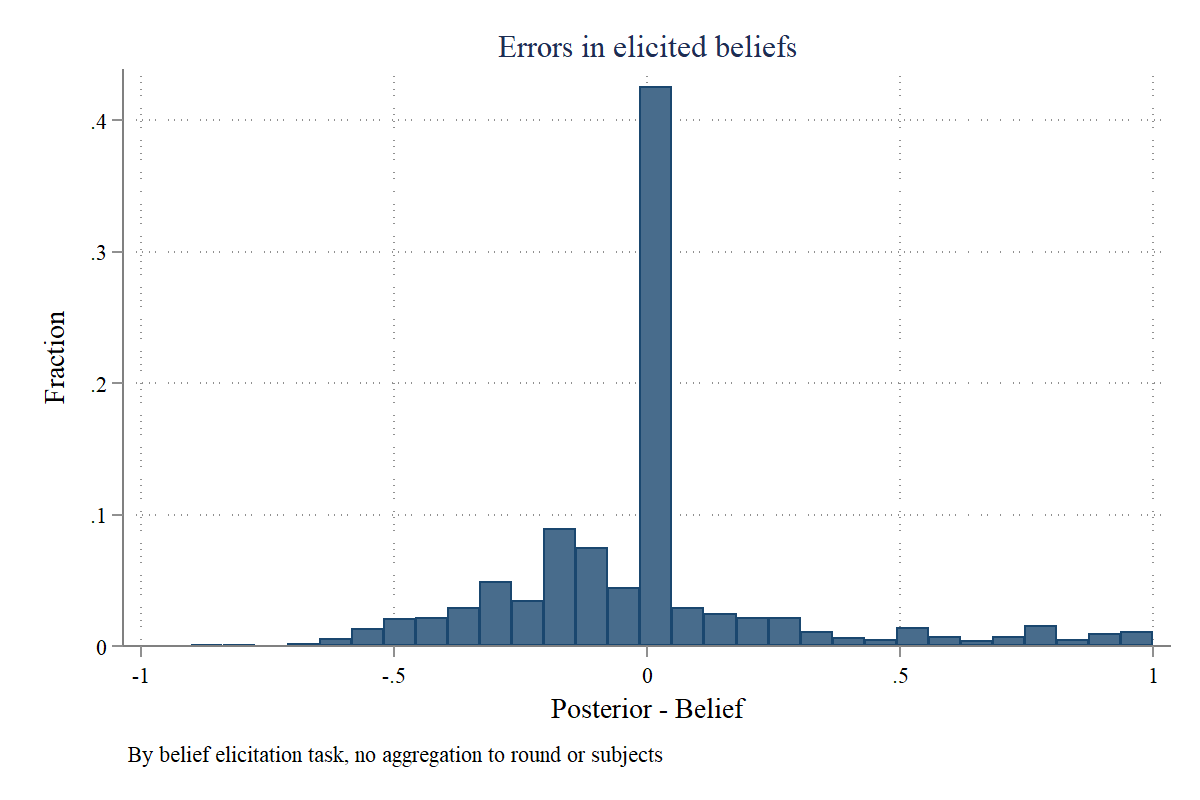
\includegraphics[width=\textwidth]{Graphs/hist_belief_error.png}
  %\caption{Belief accuracy} \label{bel_updating}
\end{subfigure}
\begin{subfigure}[t]{.48\textwidth}
  \centering
  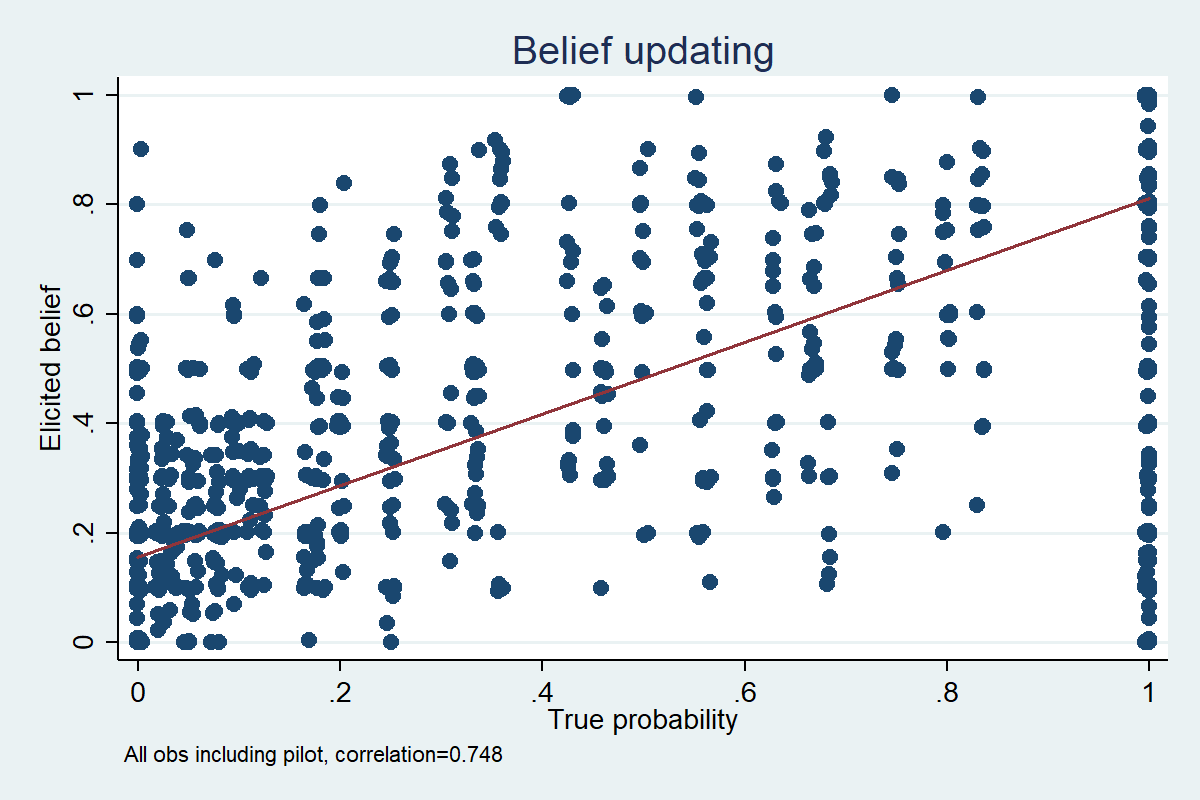
\includegraphics[width=\textwidth]{Graphs/updating_s1.png}
  %\caption{Error distribution} \label{error_hist}
\end{subfigure}

\end{figure}

\begin{figure}[!h]
\centering
\caption{Following beliefs vs following posterior probabilities in IP} \label{ref_question}
\begin{subfigure}[t]{.48\textwidth}
  \centering
  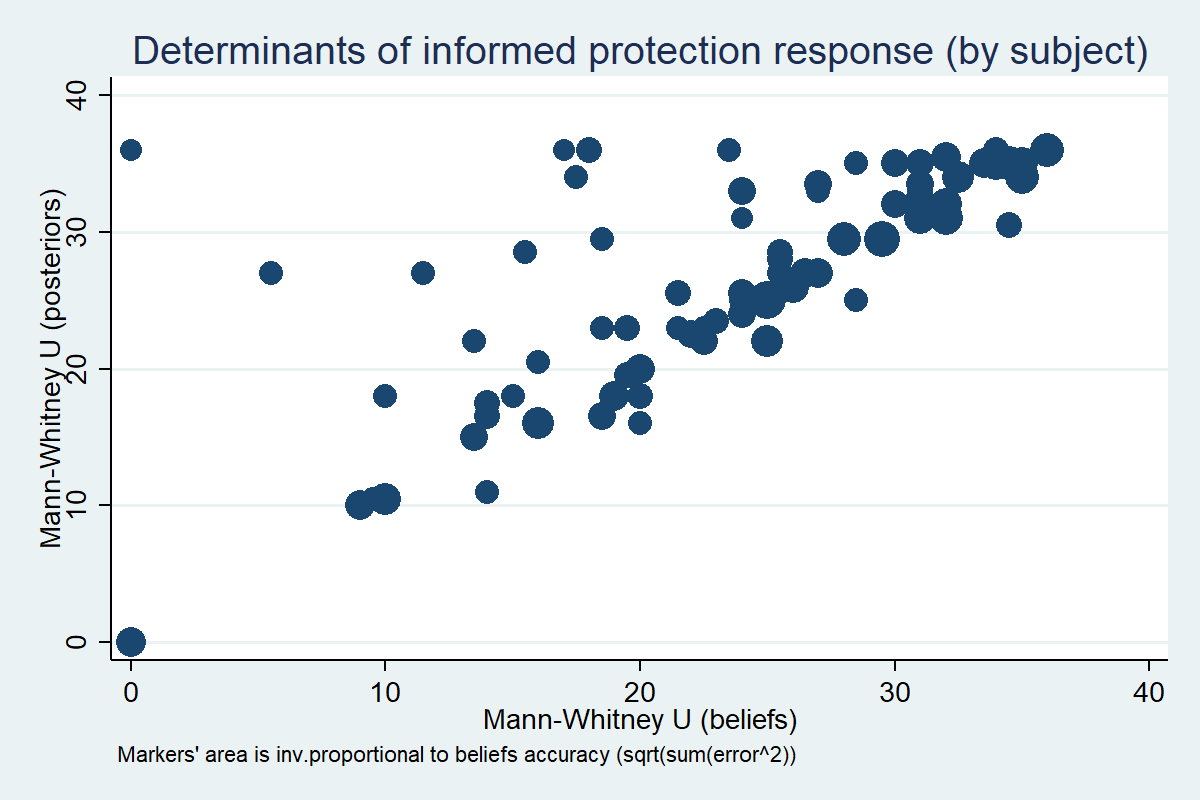
\includegraphics[width=\textwidth]{Graphs/clustering.png}
  %\caption{xx} \label{xx2}
\end{subfigure}
%\hfill
\begin{subfigure}[t]{.48\textwidth}
  \centering
  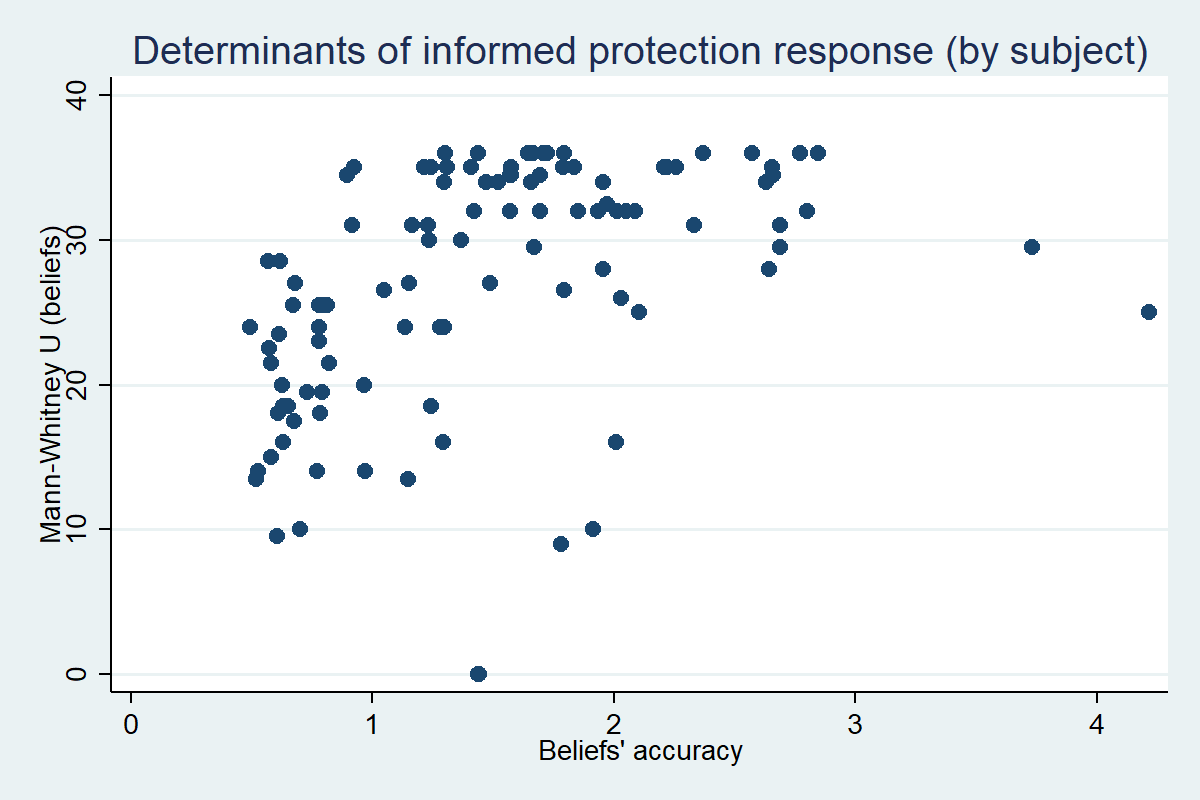
\includegraphics[width=\textwidth]{Graphs/clustering2.png}
\end{subfigure}
\end{figure}


\begin{figure}[!h]
\centering
\caption{x} \label{cost_discrepancy}

  \centering
  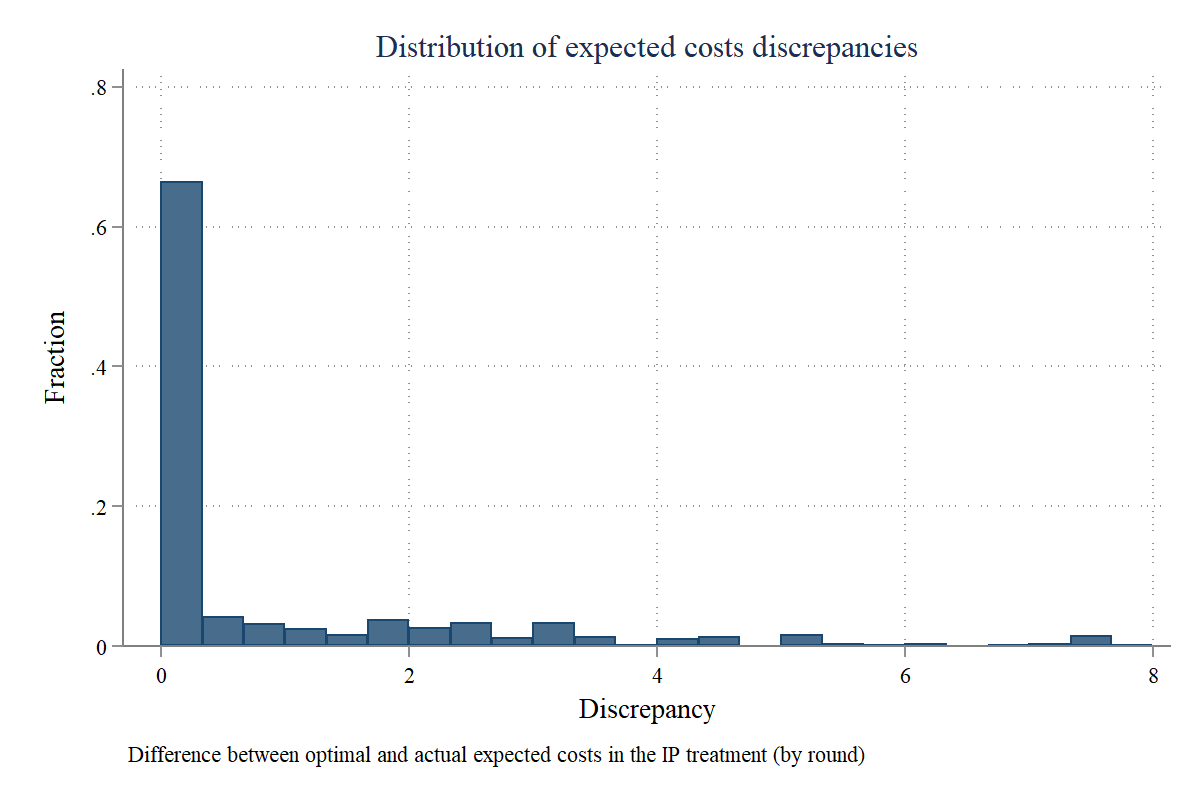
\includegraphics[width=\textwidth]{Graphs/hist_costs_discr.png}

\end{figure}




\end{document}